\chapter{Acceptance test of system}\label{app:acceptance_test}

The journal documents the acceptance test of the implemented system. The main goal of the trails is to replicate the system used in \autoref{app:journal_speaker_test} but implemented with the DSP as linkage between source and amplifier. The system is performed in a scaled environment where the the gain of the entire system is 3 dB lower than expected. This is done to protect the speaker against potential overloading.



\section{Setup}

The setup of this experiment are depicted in Figure \ref{figure:SpeakertestSetup}, where the equipment is cataloged in \autoref{tab:UsedEquipmentAcceptance}, and described as follows:

\begin{itemize}
\item Vibration and \gls{SPL} will be measured by a microphone at a distance 1 meter in accordance with IEC 60268-5 Sound System Equipment - Part 5: Loudspeaker
\item Vibration will be measured by a Brüel \& Kjear Type 4344 accelerometer, placed at the backplate of the lowest woofer.
\item The speaker will be driven by a Crown Studio Reference I amplifier.
\item The ADC/DAC will convert measurements from accelerometer and microphone and relay to a computer via SPDIF.
\item Both Accelerometer and Microphone is calibrated into outputting -35 dB at respectively 1 G and 94 dB \gls{SPL}.
\item All recordings are synchronised and timestamped by looping the test signal back into the converter.
\item The computer will be logging data with a RME HammerFall DIGI 96-PDST sound card and Adobe Audition.
\item The signal generator is a Brüel \& Kjear Type 1049 which will sweep from 2.4 kHz to 20 Hz with a speed of 80 Hz/s. Corresponding with the same signal in \autoref{app:journal_speaker_test}.
\begin{itemize}
	\item The signal will be logged in the ADC/DAC
	\item The Output from the DSP will be logged in the ADC/DAC
\end{itemize}
\item The adjustable gain for compensating the low voltage of the DSP is a Rostec LMA-4 Preamplifier.
\begin{itemize}
	\item The gain is adjusted to output 94 dB @1kHz with an input into the DSP of 0.5Volt RMS
	\item The Power amp is during calibration fixed to 6 dB.
\end{itemize}
\item The gain will be adjusted on the DSP
\end{itemize}

The reason of gain calibration is to mimic the trails made in \autoref{app:journal_speaker_test}. With the gain calibrated to same level, the DSP gain can be neglected.  Furthermore the speaker will be placed in the anechoic room to eliminate any external disturbances corresponding to the requirements demanded in the IEC 60268-5 standard.

\subsection*{Test Setup}

\begin{figure}[H]
	\centering
	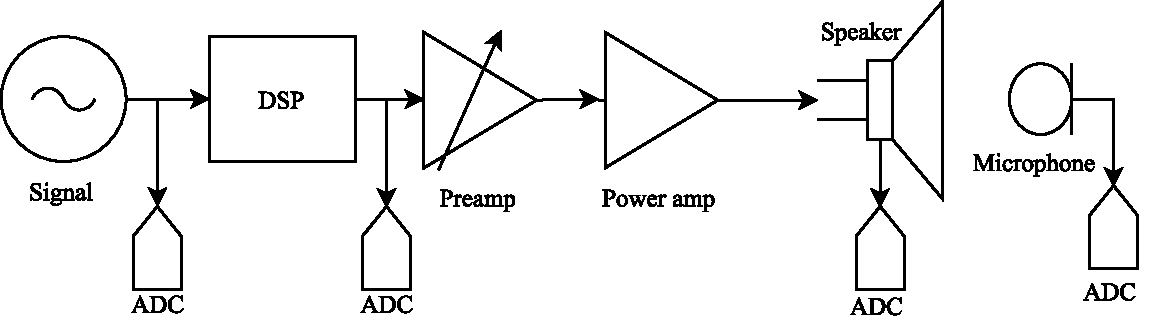
\includegraphics[width=1\textwidth]{figures/TestAcceptance}
	\caption{Schematic overview of the acceptance test setup}
	\label{fig:Acceptancetest}
\end{figure}


\subsection*{Equipment used and AAU-no.}

\begin{table}[H]
\centering
\ra{1.3}
\begin{tabular}{S[table-format=1]ccc} \toprule
    {Item} & {Description} & {AAU-no} \\ \bottomrule 
    1      &  Gras Type 40AZ microphone  & 75530   \\ 
    2      &  B \& K Accelerometer Type 4333  & 06596   \\ 
    3      &  Rostec LMA-4 Preamplifier  & 33094   \\
    4      &  Gras Type 26CC Preamplifier  & 75581   \\
    5      &  B \& K JJ2617 Accelerometer preamplifier & NaN   \\
    6      &  B \& K Power Supply 2805  & 64667  \\
    7      &  Crown Studio Reference I Amplifier & 52614   \\
    8      &  BEHRINGER digital A/D \& D/A Converter - Model ADA8000   & 56545   \\
    9      &  B \& K Accelerometer calibrator 4291 & 64668   \\
    10     &  B \& K Microphone calibrator 4231 & 78301   \\
    11     &  RME HammerFall DIGI 96-PDST sound card & 60919  \\
    12     &  Passive Dali Zensor 5 AX & NaN  \\ \bottomrule 
\end{tabular}
\caption{Table over equipment used in the test}
\label{tab:UsedEquipmentAcceptance}
\end{table}
\vspace{-5mm}


\section{Procedure}\label{sec:SpeakerTestProcedure1}

The producer for this experiment is described as follows:
\vspace{-5mm}
\begin{enumerate}
\item The poweramplifier is fixed at a gain of +19 dB
\item Vacate the anechoic room and seal the room.
\item Start recording in Adobe Audition for:
\begin{itemize}
\item Input signal and DSP output signal
\item Microphone and Accelerometer
\end{itemize}
\item Play the sweep into the dsp at following signal levels (in RMS)
\begin{enumerate}
	\item 223 mV (-7 dB)
	\item 250 mV (-6 dB)
	\item 281 mV (-5 dB)
	\item 315 mV (-4 dB)
	\item 353 mV (-3 dB)
	\item 397 mV (-2 dB)
	\item 445 mV (-1 dB)
	\item 500 mV ( 0 dB) 
\end{enumerate}
\item After sweep, stop recording all channels
\item Save recordings as \path{.wav} file
\item Repeat step 2 through 7 until the speaker breaks.
\end{enumerate}

The \path{chirp.wav} are located at:\\
\scalebox{0.7}{
\path{CD://Maalinger/Maalinger210516}}\\


%\begin{figure}[H]
%\centering
%\tikzsetnextfilename{linear_freq_sweep}
%% This file was created by matlab2tikz.
%
%The latest updates can be retrieved from
%  http://www.mathworks.com/matlabcentral/fileexchange/22022-matlab2tikz-matlab2tikz
%where you can also make suggestions and rate matlab2tikz.
%
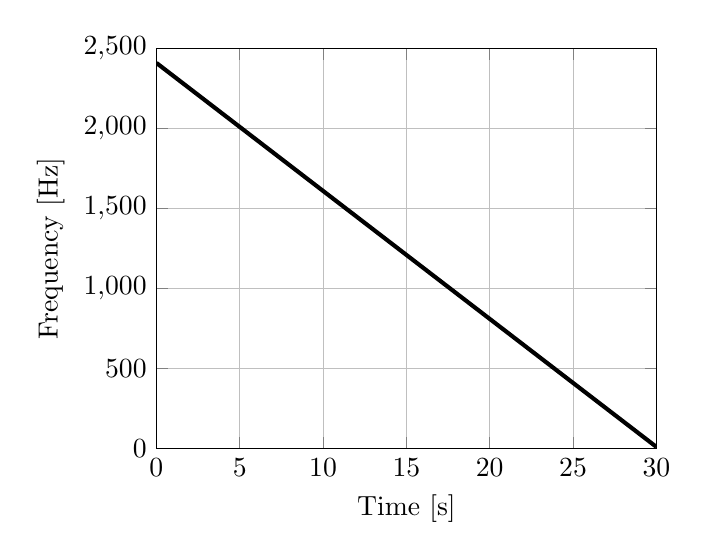
\begin{tikzpicture}

\begin{axis}[%
width=2.5in,
height=2in,
at={(1.011in,0.642in)},
scale only axis,
xmin=0,
xmax=30,
xmajorgrids,
ymin=0,
ymax=2500,
ymajorgrids,
xlabel={Time [s]},
ylabel={Frequency [Hz]},
axis background/.style={fill=white}
]
\addplot [color=black,solid,line width=1.5pt,forget plot]
  table[row sep=crcr]{%
0	2410\\
0.1	2402\\
0.2	2394\\
0.3	2386\\
0.4	2378\\
0.5	2370\\
0.6	2362\\
0.7	2354\\
0.8	2346\\
0.9	2338\\
1	2330\\
1.1	2322\\
1.2	2314\\
1.3	2306\\
1.4	2298\\
1.5	2290\\
1.6	2282\\
1.7	2274\\
1.8	2266\\
1.9	2258\\
2	2250\\
2.1	2242\\
2.2	2234\\
2.3	2226\\
2.4	2218\\
2.5	2210\\
2.6	2202\\
2.7	2194\\
2.8	2186\\
2.9	2178\\
3	2170\\
3.1	2162\\
3.2	2154\\
3.3	2146\\
3.4	2138\\
3.5	2130\\
3.6	2122\\
3.7	2114\\
3.8	2106\\
3.9	2098\\
4	2090\\
4.1	2082\\
4.2	2074\\
4.3	2066\\
4.4	2058\\
4.5	2050\\
4.6	2042\\
4.7	2034\\
4.8	2026\\
4.9	2018\\
5	2010\\
5.1	2002\\
5.2	1994\\
5.3	1986\\
5.4	1978\\
5.5	1970\\
5.6	1962\\
5.7	1954\\
5.8	1946\\
5.9	1938\\
6	1930\\
6.1	1922\\
6.2	1914\\
6.3	1906\\
6.4	1898\\
6.5	1890\\
6.6	1882\\
6.7	1874\\
6.8	1866\\
6.9	1858\\
7	1850\\
7.1	1842\\
7.2	1834\\
7.3	1826\\
7.4	1818\\
7.5	1810\\
7.6	1802\\
7.7	1794\\
7.8	1786\\
7.9	1778\\
8	1770\\
8.1	1762\\
8.2	1754\\
8.3	1746\\
8.4	1738\\
8.5	1730\\
8.6	1722\\
8.7	1714\\
8.8	1706\\
8.9	1698\\
9	1690\\
9.1	1682\\
9.2	1674\\
9.3	1666\\
9.4	1658\\
9.5	1650\\
9.6	1642\\
9.7	1634\\
9.8	1626\\
9.9	1618\\
10	1610\\
10.1	1602\\
10.2	1594\\
10.3	1586\\
10.4	1578\\
10.5	1570\\
10.6	1562\\
10.7	1554\\
10.8	1546\\
10.9	1538\\
11	1530\\
11.1	1522\\
11.2	1514\\
11.3	1506\\
11.4	1498\\
11.5	1490\\
11.6	1482\\
11.7	1474\\
11.8	1466\\
11.9	1458\\
12	1450\\
12.1	1442\\
12.2	1434\\
12.3	1426\\
12.4	1418\\
12.5	1410\\
12.6	1402\\
12.7	1394\\
12.8	1386\\
12.9	1378\\
13	1370\\
13.1	1362\\
13.2	1354\\
13.3	1346\\
13.4	1338\\
13.5	1330\\
13.6	1322\\
13.7	1314\\
13.8	1306\\
13.9	1298\\
14	1290\\
14.1	1282\\
14.2	1274\\
14.3	1266\\
14.4	1258\\
14.5	1250\\
14.6	1242\\
14.7	1234\\
14.8	1226\\
14.9	1218\\
15	1210\\
15.1	1202\\
15.2	1194\\
15.3	1186\\
15.4	1178\\
15.5	1170\\
15.6	1162\\
15.7	1154\\
15.8	1146\\
15.9	1138\\
16	1130\\
16.1	1122\\
16.2	1114\\
16.3	1106\\
16.4	1098\\
16.5	1090\\
16.6	1082\\
16.7	1074\\
16.8	1066\\
16.9	1058\\
17	1050\\
17.1	1042\\
17.2	1034\\
17.3	1026\\
17.4	1018\\
17.5	1010\\
17.6	1002\\
17.7	994\\
17.8	986\\
17.9	978\\
18	970\\
18.1	962\\
18.2	954\\
18.3	946\\
18.4	938\\
18.5	930\\
18.6	922\\
18.7	914\\
18.8	906\\
18.9	898\\
19	890\\
19.1	882\\
19.2	874\\
19.3	866\\
19.4	858\\
19.5	850\\
19.6	842\\
19.7	834\\
19.8	826\\
19.9	818\\
20	810\\
20.1	802\\
20.2	794\\
20.3	786\\
20.4	778\\
20.5	770\\
20.6	762\\
20.7	754\\
20.8	746\\
20.9	738\\
21	730\\
21.1	722\\
21.2	714\\
21.3	706\\
21.4	698\\
21.5	690\\
21.6	682\\
21.7	674\\
21.8	666\\
21.9	658\\
22	650\\
22.1	642\\
22.2	634\\
22.3	626\\
22.4	618\\
22.5	610\\
22.6	602\\
22.7	594\\
22.8	586\\
22.9	578\\
23	570\\
23.1	562\\
23.2	554\\
23.3	546\\
23.4	538\\
23.5	530\\
23.6	522\\
23.7	514\\
23.8	506\\
23.9	498\\
24	490\\
24.1	482\\
24.2	474\\
24.3	466\\
24.4	458\\
24.5	450\\
24.6	442\\
24.7	434\\
24.8	426\\
24.9	418\\
25	410\\
25.1	402\\
25.2	394\\
25.3	386\\
25.4	378\\
25.5	370\\
25.6	362\\
25.7	354\\
25.8	346\\
25.9	338\\
26	330\\
26.1	322\\
26.2	314\\
26.3	306\\
26.4	298\\
26.5	290\\
26.6	282\\
26.7	274\\
26.8	266\\
26.9	258\\
27	250\\
27.1	242\\
27.2	234\\
27.3	226\\
27.4	218\\
27.5	210\\
27.6	202\\
27.7	194\\
27.8	186\\
27.9	178\\
28	170\\
28.1	162\\
28.2	154\\
28.3	146\\
28.4	138\\
28.5	130\\
28.6	122\\
28.7	114\\
28.8	106\\
28.9	98\\
29	90\\
29.1	82\\
29.2	74\\
29.3	66\\
29.4	58\\
29.5	50\\
29.6	42\\
29.7	34\\
29.8	26\\
29.9	18\\
30	10\\
};
\end{axis}
\end{tikzpicture}%
%\caption{}
%\label{fig:linear_freq_sweep}
%\end{figure}



\section{Data Extraction}


It was possible to increase the volume by 19 dB until the loudspeaker unit got to damaged. The gain was linear increased by 1 dB, starting at 3 dB, until the 20th test were the loudspeaker unit failed. This results in 20 usable data sets.

The recordings can be found on:\\
\scalebox{0.7}{
\path{CD://Maalinger/Maalinger030316 - Loudspeaker test/Measurements030316/}}
And is indexed in folders \scalebox{0.8}{\path{Measure_X}}, where X corresponds to the test number. Every measurements inside is denoted as:
\begin{itemize}
\item Accelerometer on driver: \scalebox{0.8}{\path{Acc driver_0XX}}
\item Accelerometer in enclosure: \scalebox{0.8}{\path{Acc enclosure_0XX}}
\item Microphone: \scalebox{0.8}{\path{Mic_0XX}}
\item Playback loop: \scalebox{0.8}{\path{Reference_0XX}}
\end{itemize}

The Script used to create all graphs are located at:\\
\scalebox{0.7}{
\path{CD://Maalinger/Maalinger030316 - Loudspeaker test/Measurements030316/MeasurementAnalysis.m}}\\
Figures used in the following \ref{subsec:Raw_data_1} and Dataset 1 though 20 can be found compiled in a combined file at:
\scalebox{0.7}{
\path{CD://Maalinger/Maalinger030316 - Loudspeaker test/Measurements030316/AlleSamlet.pdf}}


\subsection{Raw Data}

\section{Analysis}

\section{Conclusion}

\section{Error sources}

Few errors could have occurred during trials, since then only variable adjusted during between measurements were the gain of the amplifier. There were however problems with moving the setup from the control room were it was calibrated and then moved into the anechoic room. The calibration was done using an visual equalizer where the output was shown with a bar chart Hence the data should bee seen with a tolerance of +/- 0.5 dB.